\documentclass[11pt]{scrartcl}

\title{Projektplan: JBomberman}
\author{Silvan Adrian \\ Fabian Binna \\ Pascal Kistler}
\date{\today{}}

\usepackage[ngerman]{babel}
\usepackage[automark]{scrpage2}
\usepackage{hyperref}
\usepackage{color}
\usepackage[normalem]{ulem}
\usepackage{scrpage2}
\usepackage{graphicx}
\usepackage{tabularx}
\graphicspath{ {./images/} }
\pagestyle{scrheadings}

\clearscrheadfoot
\ihead{
\includegraphics[scale=0.4]{jbomberman}}
\ohead{Projekt: JBomberman}
\ifoot{DomainAnalyse: JBomberman}
\cfoot{Version: 1.03}
\ofoot{Datum: 27.05.15}
\setheadsepline{0.5pt}
\setfootsepline{0.5pt}

\usepackage{ucs}
\usepackage[utf8]{inputenc}
\usepackage[T1]{fontenc}


\begin{document}
\def\arraystretch{1.5}
\begin{titlepage}
\begin{center}
\vspace{10em}

\includegraphics[scale=2]{jbomberman}
\vspace{10em}
\end{center}
\begin{center}
\huge {Projekt: JBomberman} \\
\huge {DomainAnalyse}
\end{center}
\begin{center}
\vspace{10em}
\LARGE {Pascal Kistler} \\
\LARGE {Silvan Adrian} \\
\LARGE {Fabian Binna}
\end{center}

\end{titlepage}

\newpage
\section{Änderungshistorie}
\label{sec:Änderungen}

\begin{tabularx}{\linewidth}{l l l l}
\textbf{Datum} & \textbf{Version} & \textbf{Änderung}  & \textbf{Autor} \\
\hline
\textbf{09.03.15} & 1.00 & Erstellung des Dokuments & Gruppe \\
\textbf{20.03.15} & 1.01 & Vollendung des Dokuments & Fabian Binna \\
\textbf{06.04.15} & 1.02 & Verbesserung gemäss Reviewprotokoll & Silvan Adrian \\
\textbf{27.05.15} & 1.02 & Vorbereitung zur Abgabe & Silvan Adrian\\
\end{tabularx}

\newpage
\tableofcontents
\newpage
\section{Einführung}
\label{sec:Einführung}

\subsection{Zweck}
\label{sec:Zweck}
Dieses Dokument beschreibt die Domainanalyse für das Projekt JBomberman.

\subsection{Gültigkeit}
\label{sec:Gültigkeit}
Dieses Dokument ist während des ganzen Projekts gültig und wird laufend aktualisiert.

\subsection{Übersicht}
\label{sec:Übersicht}
Dieses Dokument soll eine erste Analyse der Software zeigen. 
Das Strukturdiagramm stellt die wichtigsten Klassen dar,
 die miteinander interagieren müssen. Das Systemsequenzdiagramm 
 beschreibt die wichtigsten Abläufe der Use Cases.

\newpage
\section{DomainModell}
\label{sec:DomainModell}
\subsection{Strukturdiagramm}
\label{sec:Strukturdiagramm}

\begin{center}
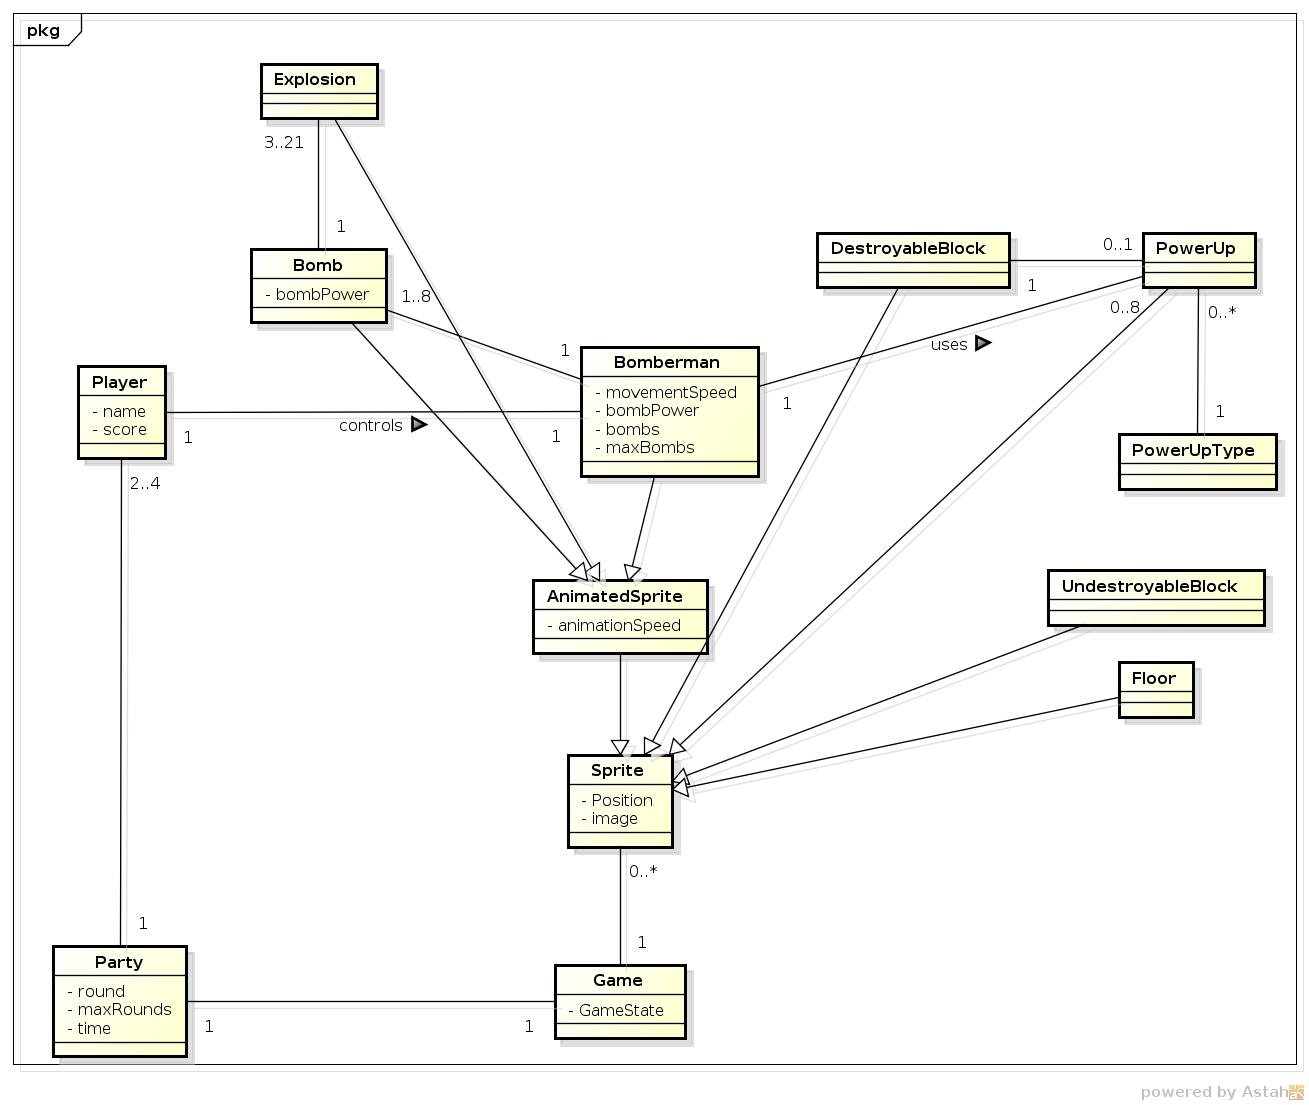
\includegraphics[scale=0.5]{Strukturdiagramm_JBomberman} 
\end{center}

\newpage
\section{Systemsequenzdiagramme}
\label{sec:Systemsequenzdiagramme}
\subsection{UC01: Bomberman spielen}
\label{sec:UC01: Bomberman spielen}
\begin{center}
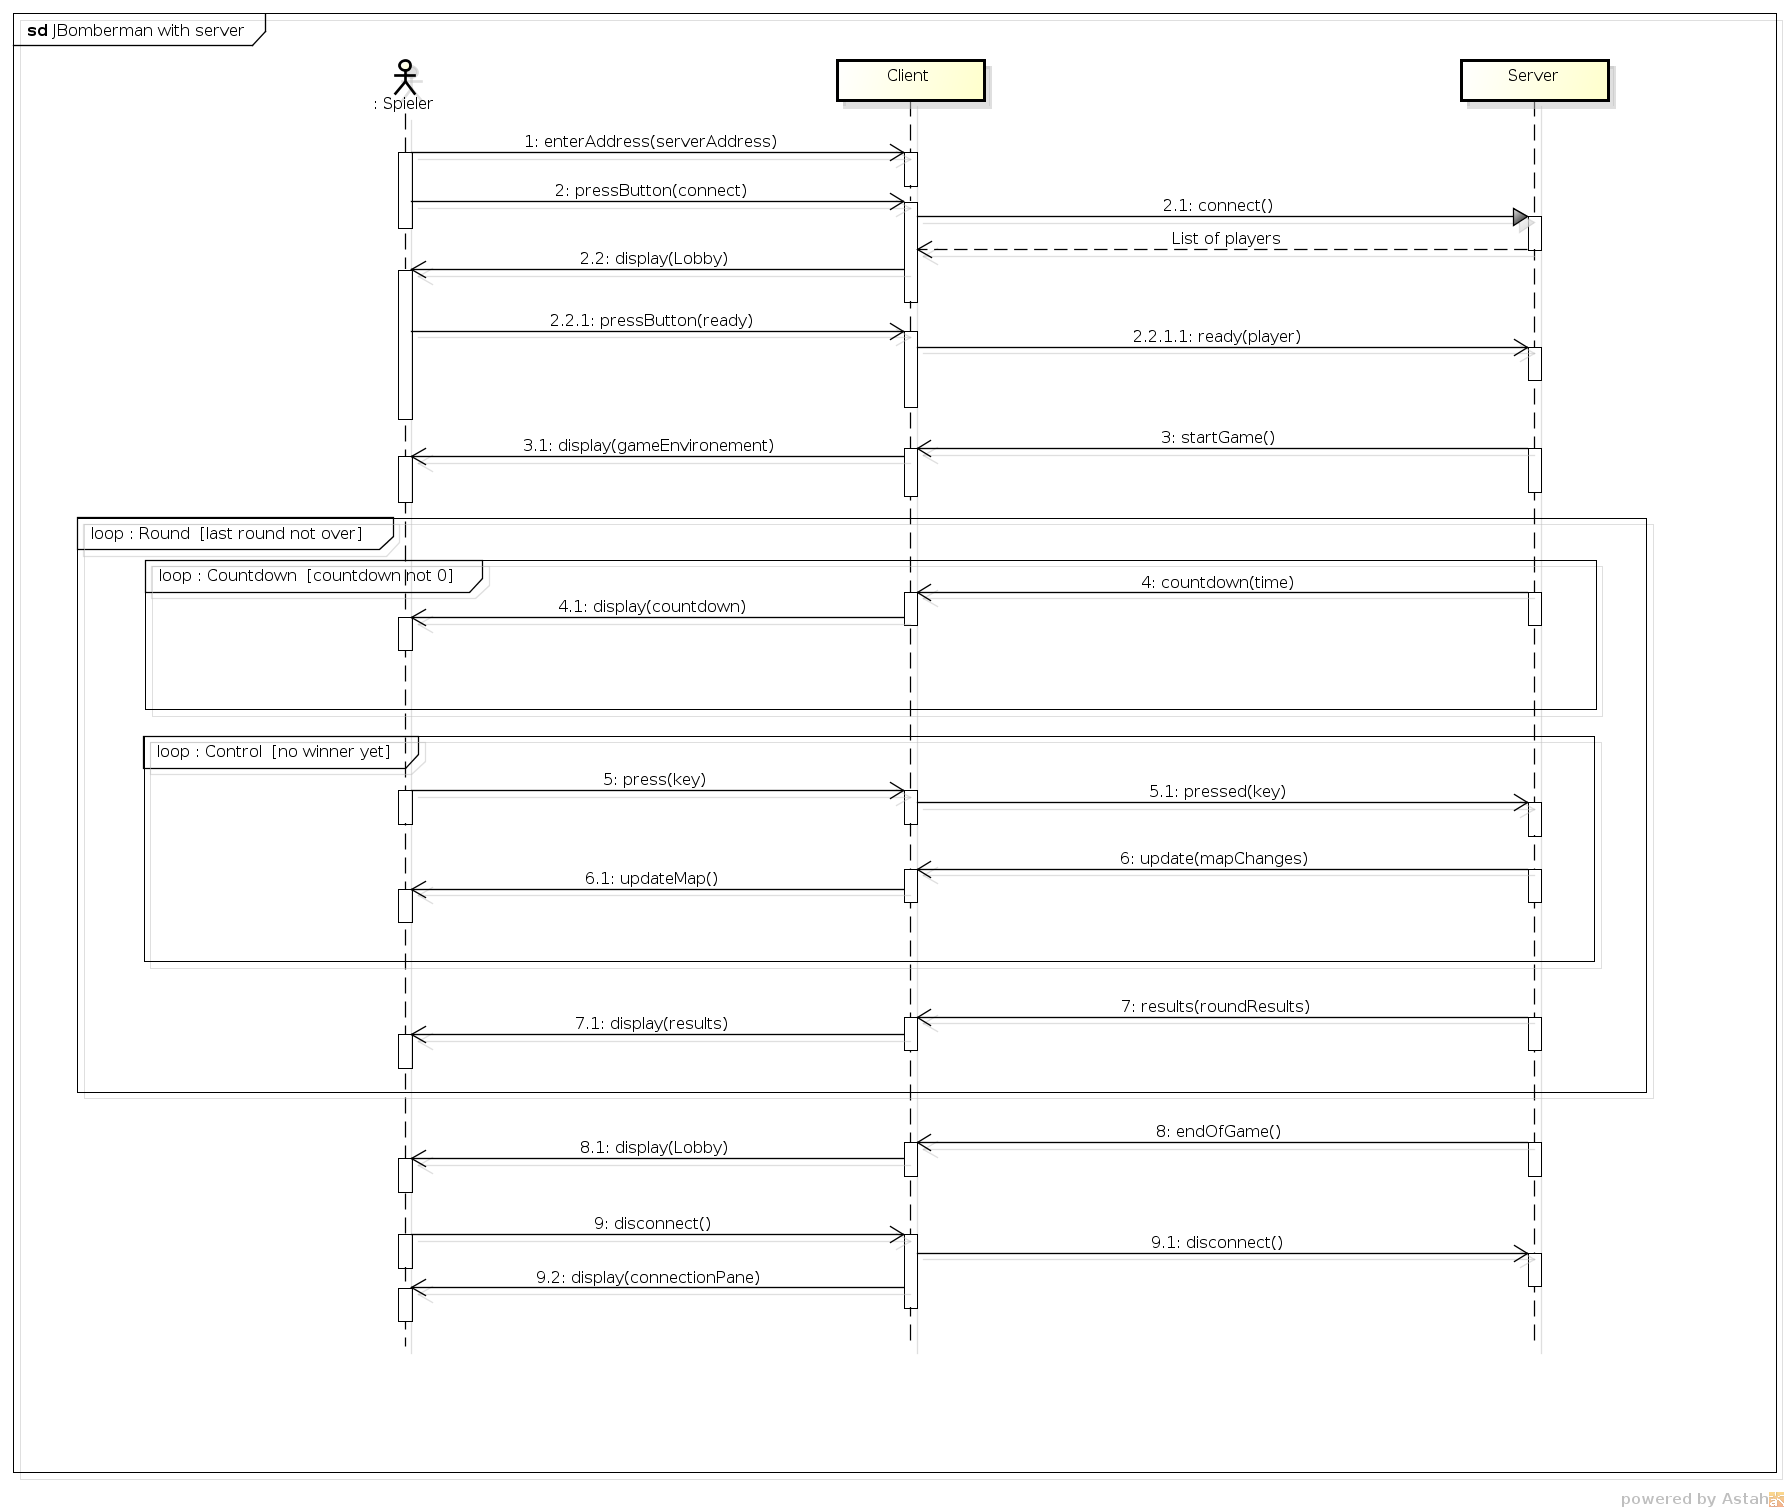
\includegraphics[scale=0.3]{SystemSequenzDiagramm_JBomberman} 
\end{center}

\newpage
\section{Systemoperationen}
\label{sec:Systemoperationen}
\subsection{Client}
\begin{itemize}
\item connect(server: Address)
\item ready(player: Player)
\item pressed(key: Message)
\item disconnect()
\end{itemize}

\subsection{Server}
\begin{itemize}
    \item startGame()
    \item countdown(time: integer)
    \item update(mapChanges: Message)
    \item results(results: Array)
    \item endOfGame()
\end{itemize}


\subsection{Contracts}
\label{sec:Contracts}

\begin{tabularx}{\linewidth}{l X}
	\textbf{Operation} & connect(server : Address) \\
	\hline
	\textbf{Cross References} & UC01 \\
	\hline
	\textbf{Preconditions} & Eine Serveradressse wurde eingegeben \\
	\hline
	\textbf{Postconditions} & 
	\begin{minipage}{5in}
		\vskip 4pt
		\begin{itemize}
			\item Der Client ist mit dem Server verbunden
			\item Der Server kennt den Client
		\end{itemize}
		\vskip 4pt
	\end{minipage}  \\
\end{tabularx}
\\ \\
\begin{tabularx}{\linewidth}{l X}
	\textbf{Operation} & ready(player : Player) \\
	\hline
	\textbf{Cross References} & UC01 \\
	\hline
	\textbf{Preconditions} & Der Client befindet sich in der Lobby \\
	\hline
	\textbf{Postconditions} & 
	\begin{minipage}{4in}
		\vskip 4pt
		\begin{itemize}
			\item Der Status des Clients wurde auf dem Server auf \textbf{ready} gesetzt
		\end{itemize}
		\vskip 4pt
	\end{minipage}  \\
\end{tabularx}
\\ \\
\begin{tabularx}{\linewidth}{l X}
	\textbf{Operation} & startGame() \\
	\hline
	\textbf{Cross References} & UC01 \\
	\hline
	\textbf{Preconditions} & Alle Client sind ready \\
	\hline
	\textbf{Postconditions} & 
	\begin{minipage}{4in}
		\vskip 4pt
		\begin{itemize}
			\item Bei den Clients wurde die Spielumgebung gestartet
			\item Der Server befindet sich im Gamemode
		\end{itemize}
		\vskip 4pt
	\end{minipage}  \\
\end{tabularx}
\\ \\
\begin{tabularx}{\linewidth}{l X}
	\textbf{Operation} & countdown(time : integer) \\
	\hline
	\textbf{Cross References} & UC01 \\
	\hline
	\textbf{Preconditions} & Das Spiel wurde gestartet \\
	\hline
	\textbf{Postconditions} & 
	\begin{minipage}{4in}
		\vskip 4pt
		\begin{itemize}
			\item Ein Countdown wird den Spielern angezeigt
		\end{itemize}
		\vskip 4pt
	\end{minipage}  \\
\end{tabularx}
\\ \\
\begin{tabularx}{\linewidth}{l X}
	\textbf{Operation} & pressed(key : Message) \\
	\hline
	\textbf{Cross References} & UC01 \\
	\hline
	\textbf{Preconditions} & Der Client befindet sich im Spiel und der Countdown ist abgelaufen \\
	\hline
	\textbf{Postconditions} & 
	\begin{minipage}{4in}
		\vskip 4pt
		\begin{itemize}
			\item Der Event ist beim Server angekommen
			\item Der Event befindet sich in der Eventqueue
		\end{itemize}
		\vskip 4pt
	\end{minipage}  \\
\end{tabularx}
\\ \\
\begin{tabularx}{\linewidth}{l X}
	\textbf{Operation} & update(mapChanges : Message) \\
	\hline
	\textbf{Cross References} & UC01 \\
	\hline
	\textbf{Preconditions} & Der Client befindet sich im Spiel \\
	\hline
	\textbf{Postconditions} & 
	\begin{minipage}{4in}
		\vskip 4pt
		\begin{itemize}
			\item Die Informationen über Änderungen in der Map wurden an den Client übertragen
			\item Der Client hat seine Map angepasst
		\end{itemize}
		\vskip 4pt
	\end{minipage}  \\
\end{tabularx}
\\ \\
\begin{tabularx}{\linewidth}{l X}
	\textbf{Operation} & results(results : Array) \\
	\hline
	\textbf{Cross References} & UC01 \\
	\hline
	\textbf{Preconditions} & Die Runde ist vorbei \\
	\hline
	\textbf{Postconditions} & 
	\begin{minipage}{4.8in}
		\vskip 4pt
		\begin{itemize}
			\item Die Clients haben die Rangliste erhalten
			\item Die Clients zeigen die Rangliste an
		\end{itemize}
		\vskip 4pt
	\end{minipage}  \\
\end{tabularx}
\\ \\
\begin{tabularx}{\linewidth}{l X}
	\textbf{Operation} & endOfGame() \\
	\hline
	\textbf{Cross References} & UC01 \\
	\hline
	\textbf{Preconditions} & Alle Runden sind vorbei \\
	\hline
	\textbf{Postconditions} & 
	\begin{minipage}{4in}
		\vskip 4pt
		\begin{itemize}
			\item Alle Clients wurden über das Ende des Spiels informiert
			\item Die Clients zeigen die Rangliste an
		\end{itemize}
		\vskip 4pt
	\end{minipage}  \\
\end{tabularx}
\\ \\
\begin{tabularx}{\linewidth}{l X}
	\textbf{Operation} & disconnect() \\
	\hline
	\textbf{Cross References} & UC01 \\
	\hline
	\textbf{Preconditions} & Der Client befindet sich in der Lobby \\
	\hline
	\textbf{Postconditions} & 
	\begin{minipage}{4in}
		\vskip 4pt
		\begin{itemize}
			\item Der Client ist nicht mehr mit dem Server verbunden
			\item Der Server hat den Client aus der Clientliste entfernt
		\end{itemize}
		\vskip 4pt
	\end{minipage}  \\
\end{tabularx}

\end{document}